\documentclass[11pt]{article}
\usepackage[T1]{fontenc}
\usepackage{lmodern}
\usepackage[margin=1in]{geometry}
\usepackage{amsmath,amssymb,amsthm}
\usepackage{microtype}
\usepackage{flafter}
\usepackage{tikz}
\usetikzlibrary{arrows.meta,positioning}
\usepackage[colorlinks=true,linkcolor=blue!45!black,citecolor=blue!45!black,urlcolor=blue!45!black]{hyperref}
\hypersetup{pdftitle={A superquadratic separation between sensitivity and block sensitivity},pdfauthor={OpenAI}}
\newcommand{\bs}{\operatorname{bs}}
\newtheorem{theorem}{Theorem}[section]
\newtheorem{lemma}[theorem]{Lemma}
\newtheorem{proposition}[theorem]{Proposition}
\newtheorem{corollary}[theorem]{Corollary}
\theoremstyle{definition}
\newtheorem{definition}[theorem]{Definition}
\theoremstyle{remark}
\newtheorem{remark}[theorem]{Remark}
\title{A superquadratic separation between sensitivity\\and block sensitivity}
\author{OpenAI}
\date{September 25, 2026}
\begin{document}
\maketitle
\begin{abstract}
We disprove the quadratic strengthening of the Sensitivity Conjecture by
constructing nonconstant total Boolean functions whose block sensitivity grows
faster than any constant multiple of sensitivity squared. In fact, for some
fixed \(\alpha>2\), our examples have unbounded block sensitivity and satisfy
\(\bs(f)\ge s(f)^\alpha\).
\end{abstract}
\section{Introduction}
\label{sec:introduction}

Sensitivity measures how many individual input bits can change a Boolean
function's value; block sensitivity allows disjoint sets of bits to be
flipped instead. We construct total Boolean functions for which the second
quantity grows faster than any constant multiple of the square of the first.

For a positive integer \(n\), write \([n]=\{1,\ldots,n\}\).
If \(x\in\{0,1\}^n\) and \(B\subseteq[n]\), let \(x^B\) be obtained
by flipping precisely the coordinates in \(B\); abbreviate
\(x^{\{a\}}\) to \(x^a\).
For a total Boolean function \(f:\{0,1\}^n\to\{0,1\}\), define
\[
 s(f,x)=\bigl|\{a\in[n]:f(x^a)\ne f(x)\}\bigr|,
 \qquad s(f)=\max_x s(f,x).
\]
Its block sensitivity \(\bs(f,x)\) is the largest number of pairwise
disjoint nonempty sets \(B_1,\ldots,B_m\subseteq[n]\) such that
\(f(x^{B_j})\ne f(x)\) for every \(j\), and
\(\bs(f)=\max_x\bs(f,x)\).

The Sensitivity Conjecture asked whether block sensitivity is bounded by a
polynomial in sensitivity, uniformly over the number of inputs and the
function. The question goes back to Nisan's work on parallel computation,
which introduced block sensitivity and already recorded Rubinstein's
quadratic separation \cite[Section~2]{Nisan1989}.
Nisan and Szegedy studied the problem through the degree of the unique
multilinear real polynomial representing a Boolean function, and explicitly
suggested the quadratic inequality \(\bs(f)\le s(f)^2\)
\cite[Section~4]{NisanSzegedy1994}.
Rubinstein's construction \cite{Rubinstein1995} showed that a polynomial
upper bound would need degree at least two. Virza improved the separation
to \(\bs(f)=\tfrac12s(f)^2+\tfrac12s(f)\) \cite{Virza2011}, and
Ambainis and Sun subsequently obtained examples satisfying
\[
 \bs(f)=\frac23s(f)^2-\frac13s(f)
\]
\cite[Theorem~1]{AmbainisSun2011}.
These improvements left open whether any universal quadratic upper bound
could hold.

Huang resolved the polynomial conjecture in 2019. His degree bound,
together with Tal's refinement of the degree--block-sensitivity comparison
\cite{Tal2013}, gives \(\bs(f)\le s(f)^4\) for every total Boolean function
\cite[Theorem~1.5]{Huang2019}. Wellens later improved its leading constant,
proving
\(\bs(f)\le\sqrt{2/3}\,s(f)^4+1\)
\cite[Corollary~4.2]{Wellens2022}.
These results settle the polynomial question. The theorem below rules out
its quadratic strengthening.

\begin{theorem}\label{thm:main}
For every real \(C>0\), there are a positive integer \(n\) and a
nonconstant total Boolean function \(f:\{0,1\}^n\to\{0,1\}\) such that
\[
 \bs(f)>C\,s(f)^2.
\]
More precisely, for every integer \(d\ge1\) the construction below gives
a nonconstant total Boolean function \(f\) with
\[
 \frac{\bs(f)}{s(f)^2}\ge \frac{2^d}{4(d+2)^2}.
\]
\end{theorem}

\paragraph{Method and relation to spectral sensitivity.}
Meiburg's spectral-sensitivity construction uses tournament-indexed rows
of positive conditions and one selected blocking coordinate in each
outgoing row \cite[Sections~3.1 and~5.2--5.5]{Meiburg2026}.\footnote{In the
attribution accompanying this construction, Meiburg credits GPT-5.6-Sol
with the gated-tournament ideas and describes his own contributions as
exposition, size and parameter optimization, and checking the faithfulness
of the Lean formalization.}
Random labels exclude small local configurations in which many accepting
subcubes lie close to the same accepting input. We adapt this architecture
to nested predicates, using a different forbidden-label condition and a
direct union bound. Simultaneous changes of two predicates then control
ordinary sensitivity under recursion.

The distinction between the two sensitivity measures matters here.
The sensitivity graph joins adjacent cube inputs exactly when the function
changes value. Its maximum degree is \(s(f)\); spectral sensitivity
\(\lambda(f)\) is the operator norm of its adjacency matrix
\cite{AaronsonEtAl2021}.
Since \(\lambda(f)\le s(f)\), a lower bound on
\(\bs(f)/\lambda(f)^2\) alone does not supply the ordinary-sensitivity
separation in Theorem~\ref{thm:main}.
The needed estimates are proved directly below, without a spectral input.

\paragraph{Construction and proof strategy.}
We recursively construct nested families of Boolean predicates: their
accepting sets decrease as the predicate index increases. At a recursive
step, the input is partitioned into disjoint child inputs arranged in
rows, and every pair of rows is given one directed edge. Each edge is
labelled by a position in its destination row. A clause associated with
row \(i\) has target conditions requiring the strongest child predicate
to accept every child in that row. For each edge from \(i\) to another row,
it also requires a weaker child predicate to reject the child selected by
the edge label. The parent predicate accepts when one of these clauses
holds. Varying the weaker predicate used in these gate conditions produces
a new nested family.

Fix one parent predicate at a rejecting input, and consider clauses that
can become satisfied after one bit changes. A bit belongs to only one child
and hence affects only one condition of a fixed clause. The candidate
clauses therefore fail exactly one target condition or one gate condition,
and no other condition. The edge labels bound the number of candidates of
the first kind. The tournament allows at most three candidates of the
second kind, and all but at most one have their failed gate in a row whose
strongest child predicates all accept. Repairing such a gate must reverse
both its weaker predicate and the strongest predicate on the same child.
We consequently track the number of bits that reverse a fixed pair of
distinct predicates simultaneously, in addition to ordinary sensitivity.
For a gate repair that makes a clause hold for two rejecting parent
predicates, the two corresponding child gate predicates must both change,
even in the possible exceptional clause.

The initial family consists of indicators of unions of Hamming balls
with successive integer radii around separated centres. One bit cannot
cross two of these radii, so all its joint sensitivities vanish.
Section~\ref{sec:construction} gives this family, the required edge
labelling, and common disjoint sensitive blocks at zero.
Section~\ref{sec:recurrences} then proves the four coupled sensitivity
bounds for arbitrary inputs. With a size parameter \(M\) chosen
sufficiently large for each fixed depth, their normalization in
Section~\ref{sec:separation} bounds sensitivity growth by essentially
a factor \(M\) per level, while the number of disjoint sensitive blocks
grows by \(2M^2+1\). An OR of disjoint copies balances the sensitivities
at zero and one, following the principle used by Ambainis and Sun
\cite[Section~4, Lemma~1]{AmbainisSun2011}.

Finally, Lemma~\ref{lem:composition} amplifies a fixed seed with
\(f(0)=0\) and \(\bs(f,0)>s(f)^2\) into the fixed power separation of
Corollary~\ref{cor:power-separation}. Ambainis and Pr\={u}sis explicitly
noted that a seed with block sensitivity greater than sensitivity squared
would yield a superquadratic power separation by iteration
\cite[Section~1]{AmbainisPrusis2014}. Composition as an amplification method
is treated systematically by Tal~\cite{Tal2013}; we prove the sensitivity
upper bound and zero-input block lower bound used here.

\section{The labelled tournament and nested predicates}
\label{sec:construction}

We construct the recursive predicates and the blocks that will witness their
block sensitivity at zero. The sensitivity estimates require control at
every input, so we also define the ordinary and joint profiles passed from
one level to the next.

Fix integers \(d\ge1\) and \(M\ge3\), and put
\[
 L=d+2,\qquad k=2M^2+1,\qquad r=\lceil\sqrt M\rceil,
 \qquad t=16.
\]
We will choose \(M\) as a function of \(d\) in
Section~\ref{sec:separation}.
A tournament is an orientation of every pair of distinct vertices:
exactly one of \(i\to j\) and \(j\to i\) holds.
Use a tournament on \([k]\) in which every vertex has outdegree \(M^2\).
For example, place the vertices cyclically and direct an edge from
each vertex to the next \(M^2\) vertices.

The tournament rows and selected blocking coordinates adapt the architecture
of Meiburg~\cite[Sections~3.1 and~5.2--5.5]{Meiburg2026}.
The specific label property needed for the ordinary-sensitivity argument is
the following elementary consequence of independent random labels.

\begin{lemma}\label{lem:labelling}
The edges can be labelled by numbers \(a(i,j)\in[r]\) so that there is
no set \(I\subseteq[k]\) of size \(t\) admitting choices
\(m_j\in[r]\), \(j\in I\), with
\[
 a(i,j)=m_j \qquad\text{for every edge }i\to j\text{ within }I.
\]
\end{lemma}
\begin{proof}
Choose all edge labels independently and uniformly from \([r]\).
For fixed \(I\) and fixed choices \((m_j)_{j\in I}\), the probability
of all the stated equalities is \(r^{-\binom t2}\).
There are at most \(k^t r^t\) choices to consider, so the probability
of any violation is at most
\[
 k^{16}r^{-104}\le (3M^2)^{16}(\sqrt M)^{-104}
 =3^{16}M^{-20}<1.
\]
Here \(k\le3M^2\), \(r\ge\sqrt M\), and \(M\ge3\).
Thus a labelling with the required property exists.
\end{proof}

Fix such a labelling for the remainder of the construction.
For \(0\le\ell\le d\), set
\[
 H_\ell=d+1-\ell,\qquad N_\ell=LM(kr)^\ell.
\]
We construct predicates \(P_{\ell,q}:\{0,1\}^{N_\ell}\to\{0,1\}\),
\(1\le q\le H_\ell\), that are nested in the sense that
\[
 P_{\ell,1}(x)\ge P_{\ell,2}(x)\ge\cdots
 \ge P_{\ell,H_\ell}(x)\quad\text{for every }x.
\]
Throughout, nesting concerns the predicate index, not the input bits.

\subsection{Initial predicates}
Partition \([LM]\) into \(M\) blocks \(E_1,\ldots,E_M\), each of
size \(L\). Let \(z_j\) be the string that is one precisely on \(E_j\).
Write \(\operatorname{dist}(x,z)\) for Hamming distance and set
\[
 D(x)=\min_{j\in[M]}\operatorname{dist}(x,z_j),\qquad
 P_{0,q}(x)=\mathbf1\{D(x)\le H_0-q\}.
\]
These predicates are nested. Their radii are the integers from \(d\)
down to zero, while distinct centres have distance \(2L=2d+4\).

\subsection{Recursive clauses}
Suppose \(1\le\ell\le d\). Partition the input into \(kr\) disjoint
children \(x_{j,c}\in\{0,1\}^{N_{\ell-1}}\), arranged in \(k\) rows
\(j\in[k]\), each with \(r\) positions \(c\in[r]\).
For this level put \(H=H_\ell\) and \(Q=H+1=H_{\ell-1}\).
For \(q\in[H]\), let clause \(i\) at index \(q\) assert
\begin{equation}\label{eq:predicate-definition}
 \begin{aligned}
 P_{\ell-1,Q}(x_{i,c})&=1 &&\text{for all }c\in[r],\\
 P_{\ell-1,Q-q}(x_{j,a(i,j)})&=0 &&\text{for all }i\to j.
 \end{aligned}
\end{equation}
Call the first line its \emph{target conditions} and the second line
its \emph{gate conditions}. Figure~\ref{fig:clause} depicts the target row
and one outgoing gate. Define \(P_{\ell,q}(x)=1\) if at least
one clause is satisfied, and zero otherwise. All indices are valid:
\(1\le Q-q\le H<Q\).
Within a single clause, all \(r+M^2\) conditions use distinct children.
Indeed, targets use row \(i\), each gate uses another row, and there
is only one edge from \(i\) to any given row. Consequently a change
of one raw input bit can affect at most one condition of that clause.
The same bit can affect several clauses, which will cause no problem
when taking upper bounds by unions of sets of bits.

By induction, increasing \(q\) makes each gate condition stronger:
the index \(Q-q\) decreases, and requiring a larger nested predicate
to be zero is more restrictive. Targets do not change. Thus each
clause, and hence each \(P_{\ell,q}\), is nested as asserted.
This recursion defines total Boolean functions on exactly
\(N_\ell=krN_{\ell-1}\) bits.

\begin{figure}[htbp]
\centering
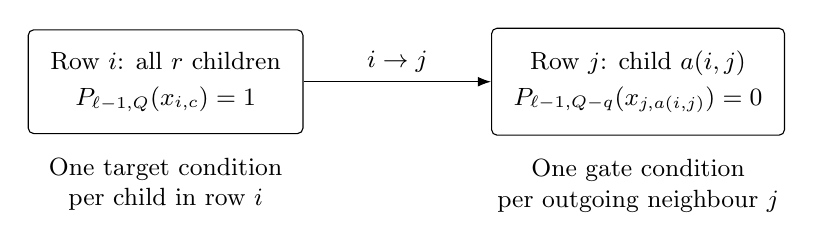
\begin{tikzpicture}[>=Latex, every node/.style={font=\small},
  condition/.style={draw,rounded corners=2pt,inner sep=8pt,align=center}]
 \node[condition] (target) at (0,0)
   {Row \(i\): all \(r\) children\\[2pt]
    \(P_{\ell-1,Q}(x_{i,c})=1\)};
 \node[condition] (gate) at (6,0)
   {Row \(j\): child \(a(i,j)\)\\[2pt]
    \(P_{\ell-1,Q-q}(x_{j,a(i,j)})=0\)};
 \draw[->] (target) -- node[above]{\(i\to j\)} (gate);
 \node[below=5pt of target,align=center] {One target condition\\per child in row \(i\)};
 \node[below=5pt of gate,align=center] {One gate condition\\per outgoing neighbour \(j\)};
\end{tikzpicture}
\caption{One recursive clause. The edge label selects a single child in
each outgoing neighbour's row. Raising \(q\) strengthens the gates;
all targets use the strongest child predicate \(Q\).}
\label{fig:clause}
\end{figure}

\subsection{Sensitivity profiles and the initial bounds}
For \(b\in\{0,1\}\), define
\[
 S_{\ell,b}=\max_{\substack{1\le q\le H_\ell,\ x\in\{0,1\}^{N_\ell}\\
                           P_{\ell,q}(x)=b}}
 \bigl|\{a\in[N_\ell]:P_{\ell,q}(x^a)=1-b\}\bigr|.
\]
We also keep track of simultaneous changes of two distinct predicates:
\[
 J_{\ell,b}=\max_{\substack{1\le q<q'\le H_\ell,\ x\in\{0,1\}^{N_\ell}\\
                         P_{\ell,q}(x)=P_{\ell,q'}(x)=b}}
 \bigl|\{a\in[N_\ell]:P_{\ell,q}(x^a)=P_{\ell,q'}(x^a)=1-b\}\bigr|.
\]
A maximum over no cases is defined to be zero; in particular
\(J_{d,0}=J_{d,1}=0\), since \(H_d=1\).
The two predicates in the definition of \(J_{\ell,b}\) are evaluated
on the same input and changed by the same raw input bit.

\begin{lemma}\label{lem:base}
The initial sensitivity profiles satisfy
\begin{equation}\label{eq:base-profile}
 S_{0,0}\le L,\qquad S_{0,1}\le LM,\qquad
 J_{0,0}=J_{0,1}=0.
\end{equation}
\end{lemma}
\begin{proof}
Fix a predicate of radius \(R=H_0-q\in\{0,\ldots,d\}\) and an
input \(x\) at which it is zero. If flipping one bit makes it one,
some centre must be at distance exactly \(R+1\) from \(x\).
There is at most one centre within distance \(d+1\) of \(x\):
two such centres would have distance at most \(2d+2<2L\).
Thus every successful bit flip must move towards the same centre,
giving at most \(R+1\le d+1\le L\) possibilities.
The bound on \(S_{0,1}\) is simply the number \(LM\) of input bits.

For adjacent inputs \(x,y\), the triangle inequality gives
\(D(x)\le D(y)+1\), and the reverse inequality follows by symmetry.
Hence \(|D(x)-D(y)|\le1\). To change both predicates with distinct
integer radii from zero to one, or both from one to zero, would require
\(D\) to change by at least two. Both joint sensitivities are therefore
zero.
\end{proof}

\subsection{Disjoint blocks at zero}
\begin{lemma}\label{lem:blocks}
At every level \(0\le\ell\le d\), all predicates are zero at the
all-zero input. There are \(Mk^\ell\) pairwise disjoint nonempty blocks
of coordinates, each of size \(Lr^\ell\), such that flipping any one
block at zero makes every predicate at that level equal to one.
\end{lemma}
\begin{proof}
At level zero, \(D(0)=L>d\), and the blocks \(E_j\) have the stated
property because \(0^{E_j}=z_j\).
Suppose the claim holds at level \(\ell-1\). At the all-zero input,
every target predicate is zero, so every clause fails at level \(\ell\).

Enumerate the preceding-level block family as
\(B_1,\ldots,B_{Mk^{\ell-1}}\).
For each row \(i\) and each family index \(h\), take the union of the
copies of \(B_h\) in all \(r\) children of row \(i\).
Flipping this union makes the strongest predicate in each of those
children equal to one, so all targets for clause \(i\) hold.
All gate children of clause \(i\) lie in other rows and remain zero,
so its gates hold for every \(q\).
Thus every \(P_{\ell,q}\) is one after the flip.
Within a row these unions are disjoint because the preceding-level
blocks are disjoint in every child; unions from different rows are
also disjoint. There are \(k\cdot Mk^{\ell-1}=Mk^\ell\) of them,
each of size \(r\cdot Lr^{\ell-1}=Lr^\ell\), as required.
\end{proof}

\section{Sensitivity recurrences}
\label{sec:recurrences}

The joint profiles bound simultaneous changes of a fixed pair of predicates
on the same child. The following estimates hold for every input, including
inputs far from the blocks used in Lemma~\ref{lem:blocks}.

\begin{proposition}\label{prop:recurrences}
For $1\leq \ell\leq d$, write
$S'_b=S_{\ell-1,b}$ and $J'_b=J_{\ell-1,b}$.  Then
\begin{equation}\label{eq:recurrences}
\begin{aligned}
 S_{\ell,1}&\leq M^2S'_0+rS'_1,
 &\qquad J_{\ell,1}&\leq M^2J'_0+rS'_1,\\
 S_{\ell,0}&\leq tS'_0+S'_1+3J'_1,
 &\qquad J_{\ell,0}&\leq tS'_0+3J'_1.
\end{aligned}
\end{equation}
\end{proposition}

\begin{proof}
Fix $\ell$, put $H=H_\ell$ and $Q=H+1$, and recall
Equation~\eqref{eq:predicate-definition}.  For predicate index $q$, every
target tests $P_{\ell-1,Q}=1$ and every gate tests
$P_{\ell-1,Q-q}=0$ on its specified child.  The targets of clause $i$
lie in row $i$, and its gates lie in distinct other rows.  Thus each
condition of a fixed clause uses a different child.

All flips below are flips of individual coordinates of the original
Boolean input.  Such a flip affects exactly one child.  It may change
several nested predicates of that child; we make no restriction on the
number of thresholds it crosses.  Nevertheless, at a fixed parent index
it can change at most one condition of any fixed clause.  A child may
occur in several different clauses, so when counting possible flips
over clauses we use a union bound.

\emph{Transitions from one.}
Fix an input where $P_{\ell,q}=1$, and choose a clause satisfied there.
Every flip taking this predicate to zero must break that fixed clause.
It either changes a gate predicate from zero to one or changes a target
predicate from one to zero.  There are $M^2$ gate children and $r$
target children, giving at most $M^2S'_0+rS'_1$ such flips.

Next fix $q<q'$ and an input where both parent predicates are one.
Choose a clause initially satisfied for $q'$; nesting makes it satisfied
for $q$ as well.  This same clause is fixed for all flips being counted.
A flip taking both parent predicates to zero must either break one of
its targets, accounting for at most $rS'_1$ flips, or leave all its
targets true and fail a gate even for $q$.  Put
\[
 g=Q-q,\qquad g'=Q-q',\qquad 1\leq g'<g<Q.
\]
At such a gate, initially $P_{\ell-1,g'}=0$ because the clause holds
for $q'$, and nesting gives $P_{\ell-1,g}=0$.  Failure of the gate for
$q$ after the flip means $P_{\ell-1,g}=1$, and nesting then gives
$P_{\ell-1,g'}=1$.  The two distinct child predicates therefore both
change from zero to one.  Each of the $M^2$ gates contributes at most
$J'_0$ such flips.  This proves both inequalities on the one side.

\emph{The initial candidate clauses at a zero.}
Fix $q$ and an input $x$ with $P_{\ell,q}(x)=0$.  Let $\mathcal T$
be the set of clauses that at $x$ fail exactly one target and no gate,
and let $\mathcal G$ be the set that fail exactly one gate and no
target.  These sets are determined by $x$ and $q$, before a flipped
coordinate is chosen.  Every flip making $P_{\ell,q}$ one satisfies
some previously false clause.  Since only one condition of that clause
can change, the clause belongs to $\mathcal T\cup\mathcal G$, and
its unique failed condition must be repaired.

For each $j\in\mathcal T$, let $m_j\in[r]$ be the position of its
unique failed target.  If $i,j\in\mathcal T$ and $i\to j$, clause
$i$ has a passing gate in child $(j,a(i,j))$.  Its gate predicate
$P_{\ell-1,Q-q}$ is zero, so by nesting its target predicate
$P_{\ell-1,Q}$ is also zero.  The unique failed target in row $j$
is at position $m_j$, forcing $a(i,j)=m_j$.  Consequently a set of
$t$ vertices in $\mathcal T$ would violate Lemma~\ref{lem:labelling}.
Thus $|\mathcal T|<t$.  Repairing a clause in this list requires
changing its unique failed target from zero to one, and accounts for
at most $S'_0$ flips per clause.  Their total contribution is at most
$tS'_0$.

All targets in the row of a vertex of $\mathcal G$ are initially
true.  Hence an edge $i\to j$ within $\mathcal G$ gives a failed
gate of clause $i$: the gate child in row $j$ has
$P_{\ell-1,Q}=1$, which forces $P_{\ell-1,Q-q}=1$.  A clause in
$\mathcal G$ has just one failed gate, so every outdegree in the
induced tournament on $\mathcal G$ is at most one.  With
$m=|\mathcal G|$, counting its edges gives
\[
 \frac{m(m-1)}2\leq m,
 \qquad\text{and hence}\qquad m\leq3.
\]
There is at most one vertex of outdegree zero in this induced
tournament, since the edge between any two vertices leaves one of
them.

If $i\in\mathcal G$ has an outgoing edge $i\to j$ inside
$\mathcal G$, that edge is its unique failed gate.  On the
corresponding child, initially
\[
 P_{\ell-1,Q-q}=P_{\ell-1,Q}=1.
\]
Repairing the gate sets $P_{\ell-1,Q-q}=0$ and therefore also sets
$P_{\ell-1,Q}=0$.  The indices $Q-q$ and $Q$ are distinct because
$q\geq1$, so at most $J'_1$ flips repair this clause.  The fact that
such a flip destroys a target in row $j$ causes no problem: the
accepting witness is clause $i$, whose own targets and other gates
are unchanged.  The possible vertex with no outgoing edge inside
$\mathcal G$ contributes at most $S'_1$, by counting flips of its
unique failed gate.  Since $|\mathcal G|\leq3$, its entire
contribution is at most $S'_1+3J'_1$.  Together with the target
contribution this proves
$S_{\ell,0}\leq tS'_0+S'_1+3J'_1$.

\emph{Joint transitions from zero.}
Fix $q<q'$ and an input $x$ where both parent predicates are zero,
and form the same initial lists $\mathcal T,\mathcal G$ for the
weaker index $q$.  Consider a flip making both predicates one, and
choose any clause satisfied afterward for $q'$.  It is also satisfied
afterward for $q$, so it belongs to those fixed initial lists.  The
choice of this final witness may depend on the flipped coordinate;
the lists themselves do not.  A genuine final witness also had
exactly one failed condition at $q'$ initially, by the same
distinct-child argument.  Members of the weaker lists that have
additional unrepaired failures at $q'$ simply contribute no flips.

A witness in $\mathcal T$ is counted by the preceding target bound
$tS'_0$.  For a witness in $\mathcal G$, let $g=Q-q$ and
$g'=Q-q'$, so $1\leq g'<g<Q$.  Its unique failed gate at index $q$
has $P_{\ell-1,g}=1$ initially, and nesting gives
$P_{\ell-1,g'}=1$ initially as well.  To satisfy the clause for
$q'$ afterward, the same child must have $P_{\ell-1,g'}=0$, which
forces $P_{\ell-1,g}=0$.  Thus both distinct child predicates change
from one to zero, and each such clause contributes at most $J'_1$.
This reasoning applies also to the possible vertex with no outgoing
edge inside $\mathcal G$: the second parent index supplies the
second child threshold, without requiring any initial target value
at the failed gate.  The gate contribution is therefore at most
$3J'_1$.

Every joint-success coordinate is thus counted by a clause in the fixed
lists $\mathcal T$ or $\mathcal G$, so a union bound gives
$J_{\ell,0}\leq tS'_0+3J'_1$.

All bounds hold for every relevant input and for each fixed index or
pair of indices, so taking the maxima gives the proposition.  If
$H=1$, there is no pair of distinct parent indices and both joint
inequalities hold by the empty-maximum convention.
\end{proof}

\section{Quantitative bounds and separation}
\label{sec:separation}

The dominant terms $M^2S'_0$ and $S'_1$ in
Proposition~\ref{prop:recurrences} suggest normalizing $S_{\ell,b}$ by
$M^{\ell+b}$. The joint profiles vanish initially; choosing $M$ large
relative to $d$ keeps their contribution small through the prescribed
depth. The following bound makes this choice explicit.

\begin{lemma}
\label{lem:quantitative-profiles}
Suppose that $d\geq 1$ and $M\geq 9^{d+1}$.
For every $0\leq\ell\leq d$ and $b\in\{0,1\}$, the predicates of the
construction satisfy
\[
  S_{\ell,b}\leq 2L M^{\ell+b}.
\]
\end{lemma}

\begin{proof}
Define
\[
 u_\ell=\max_{b\in\{0,1\}}\frac{S_{\ell,b}}{M^{\ell+b}},
 \qquad
 v_\ell=\max_{b\in\{0,1\}}\frac{J_{\ell,b}}{M^{\ell+b}},
 \qquad
 \epsilon=\frac{\max(r,t)}{M}.
\]
The base bounds in~\eqref{eq:base-profile} give $u_0\leq L$ and $v_0=0$.
For $1\leq\ell\leq d$, dividing the four inequalities in
Proposition~\ref{prop:recurrences} by the corresponding powers of~$M$
gives
\begin{align*}
 \frac{S_{\ell,1}}{M^{\ell+1}}
   &\leq \left(1+\frac rM\right)u_{\ell-1},
 &\qquad
 \frac{S_{\ell,0}}{M^\ell}
   &\leq \left(1+\frac tM\right)u_{\ell-1}+3v_{\ell-1},\\
 \frac{J_{\ell,1}}{M^{\ell+1}}
   &\leq \frac rM u_{\ell-1}+v_{\ell-1},
 &
 \frac{J_{\ell,0}}{M^\ell}
   &\leq \frac tM u_{\ell-1}+3v_{\ell-1}.
\end{align*}
Consequently,
\begin{equation}
\label{eq:normalized-recurrences}
 \begin{split}
  u_\ell&\leq (1+\epsilon)u_{\ell-1}+3v_{\ell-1},\\
  v_\ell&\leq \epsilon u_{\ell-1}+3v_{\ell-1}.
 \end{split}
\end{equation}
The forcing term for $v_\ell$ is at most $\epsilon u_{\ell-1}$, while
its inherited contribution is multiplied by at most three. We therefore
make $\epsilon$ small compared with $3^{-d}$. Since $M\geq81$, both
$r=\lceil\sqrt M\rceil\leq2\sqrt M$ and $t=16\leq2\sqrt M$.
It follows that
\begin{equation}
\label{eq:epsilon-choice}
 \epsilon\leq\frac{2}{\sqrt M}\leq\frac{2}{3^{d+1}}.
\end{equation}

Let $U_0=L$, $V_0=0$, and define the comparison sequences by
\[
 U_\ell=(1+\epsilon)U_{\ell-1}+3V_{\ell-1},
 \qquad
 V_\ell=\epsilon U_{\ell-1}+3V_{\ell-1}.
\]
All coefficients are nonnegative, so~\eqref{eq:normalized-recurrences}
implies $u_\ell\leq U_\ell$ and $v_\ell\leq V_\ell$ by induction.
We prove simultaneously that, for $0\leq\ell\leq d$,
\begin{equation}
\label{eq:comparison-bounds}
 U_\ell\leq2L,
 \qquad
 V_\ell\leq\epsilon L(3^\ell-1).
\end{equation}
These bounds hold at $\ell=0$.
Suppose they hold at every index less than some $1\leq\ell\leq d$.
First,
\[
 V_\ell
 \leq 2\epsilon L+3\epsilon L(3^{\ell-1}-1)
 =\epsilon L(3^\ell-1).
\]
Next, summing the increments of $U_j$ and using only the bounds at
indices $j<\ell$, we obtain
\begin{align*}
 U_\ell
 &=L+\sum_{j=0}^{\ell-1}(\epsilon U_j+3V_j)\\
 &\leq L+2\epsilon L\ell
          +3\epsilon L\sum_{j=0}^{\ell-1}(3^j-1)\\
 &=L+\epsilon L\left[\frac32(3^\ell-1)-\ell\right]
 <2L.
\end{align*}
The last inequality follows from~\eqref{eq:epsilon-choice}, since
\[
 \epsilon\left[\frac32(3^\ell-1)-\ell\right]
 \leq\frac{3^{\ell+1}-3-2\ell}{3^{d+1}}<1.
\]
This completes the simultaneous induction. In particular,
$u_\ell\leq2L$, which is the desired bound.
\end{proof}

\begin{proof}[Proof of Theorem~\ref{thm:main}]
Fix any integer $d\geq1$ and choose an integer $M\geq9^{d+1}$.
Lemma~\ref{lem:labelling} provides the required tournament labels.
Following the OR-balancing principle of Ambainis and Sun
\cite[Section~4, Lemma~1]{AmbainisSun2011}, take $f$ to be the OR of $M$
disjoint copies of $P_{d,1}$.
Each copy has dimension $LM(kr)^d$, so $f$ is a total Boolean function on
\begin{equation}
\label{eq:final-dimension}
 n=LM^2(kr)^d
\end{equation}
bits. By Lemma~\ref{lem:blocks}, every copy is zero at its zero input,
and a block from its stated family makes that copy one.
Thus $f(0)=0$ and $f$ is nonconstant.

At a zero input of $f$, every copy is zero, and its sensitivity is at most
$M S_{d,0}$. At a one input, either at least two copies accept, in which
case no single bit can change the OR to zero, or exactly one copy accepts.
In the latter case every sensitive bit belongs to that accepting copy,
so there are at most $S_{d,1}$ such bits.
Lemma~\ref{lem:quantitative-profiles} therefore gives
\begin{equation}
\label{eq:final-sensitivity}
 s(f)\leq\max\{M S_{d,0},S_{d,1}\}
       \leq2L M^{d+1}.
\end{equation}

Each copy supplies $M k^d$ pairwise disjoint blocks sensitive at zero,
by Lemma~\ref{lem:blocks}. Taking their union over the disjoint copies
gives a family of $M^2k^d$ pairwise disjoint sensitive blocks for $f$ at zero.
In particular,
\begin{equation}
\label{eq:final-block-sensitivity}
 \bs(f,0)\geq M^2k^d.
\end{equation}
Since $f$ is nonconstant, $s(f)>0$. Combining
\eqref{eq:final-sensitivity} and~\eqref{eq:final-block-sensitivity} yields
\begin{equation}
\label{eq:ratio-separation}
 \frac{\bs(f)}{s(f)^2}
 \geq\frac{\bs(f,0)}{s(f)^2}
 \geq\frac{(k/M^2)^d}{4L^2}
 \geq\frac{2^d}{4(d+2)^2}.
\end{equation}
The last expression tends to infinity as $d$ tends to infinity.
For any proposed constant $C$, first choose $d$ so that this expression
exceeds $C$, then choose $M\geq9^{d+1}$, then choose labels supplied by
Lemma~\ref{lem:labelling} and form $f$ as above.
The resulting finite-dimensional total nonconstant function satisfies
$\bs(f)>C s(f)^2$. Hence no universal quadratic constant exists.
\end{proof}

\subsection{A fixed exponent by composition}

The construction also supplies a fixed seed whose block sensitivity at
zero exceeds the square of its sensitivity. Repeated composition of that
seed gives a power separation. This is the composition-and-powering
principle studied by Tal~\cite{Tal2013}. We include the elementary composition facts
to make this additional consequence self-contained.

\begin{lemma}
\label{lem:composition}
Let $f:\{0,1\}^a\to\{0,1\}$ and
$g:\{0,1\}^b\to\{0,1\}$ be total Boolean functions.
Their disjoint composition is the function on $ab$ bits defined by
\[
 (f\circ g)(x_1,\ldots,x_a)
   =f\bigl(g(x_1),\ldots,g(x_a)\bigr),
 \qquad x_i\in\{0,1\}^b.
\]
Then
\[
 s(f\circ g)\leq s(f)s(g).
\]
If $g(0)=0$, then $(f\circ g)(0)=f(0)$ and
\[
 \bs(f\circ g,0)\geq\bs(f,0)\bs(g,0).
\]
More explicitly, any disjoint families of $p$ and $q$ blocks sensitive at
zero for $f$ and $g$, respectively, yield a disjoint family of $pq$ blocks
sensitive at zero for $f\circ g$.
\end{lemma}

\begin{proof}
For an input $x=(x_1,\ldots,x_a)$, put
$y=(g(x_1),\ldots,g(x_a))$.
A bit in child $x_i$ is sensitive for $f\circ g$ precisely when it is
sensitive for $g$ at $x_i$ and coordinate $i$ is sensitive for $f$ at $y$.
Thus
\[
 s(f\circ g,x)
   =\sum_{i:\,f(y^{\{i\}})\ne f(y)}s(g,x_i)
   \leq s(f,y)s(g)
   \leq s(f)s(g).
\]

Now suppose $g(0)=0$. Let $C_1,\ldots,C_p\subseteq[a]$ and
$D_1,\ldots,D_q\subseteq[b]$ be disjoint nonempty sensitive blocks for
$f$ and $g$ at zero. Identify the coordinates of the composition with
$[a]\times[b]$. For each $1\leq i\leq p$ and $1\leq j\leq q$, set
\[
 E_{i,j}=C_i\times D_j.
\]
These blocks are nonempty and pairwise disjoint: different $i$ use
disjoint sets of children, while for fixed $i$ different $j$ use
disjoint coordinate sets in each child.
Flipping $E_{i,j}$ at zero makes precisely the children indexed by $C_i$
output one, because $g(0)=0$ and $D_j$ is sensitive there.
The outer input therefore becomes $0^{C_i}$, which changes the value of
$f$. Hence every $E_{i,j}$ is sensitive for $f\circ g$ at zero.
Choosing maximum families proves the stated block-sensitivity inequality;
if either maximum is zero, the inequality is immediate.
\end{proof}

\begin{corollary}
\label{cor:power-separation}
There exist a real number $\alpha>2$ and nonconstant total Boolean
functions $F_m$, for integers $m\geq1$, such that
\[
 \bs(F_m,0)\geq s(F_m)^\alpha
 \qquad\text{for every }m,
 \qquad
 \bs(F_m,0)\longrightarrow\infty.
\]
\end{corollary}

\begin{proof}
Fix $d=9$, choose an integer $M\geq9^{10}$, and choose any admissible
labelling. Let $f$ be the function constructed in the proof of
Theorem~\ref{thm:main} for these fixed parameters. Put
\[
 A=22M^{10},\qquad B=M^2k^9.
\]
Here $L=11$, so~\eqref{eq:final-sensitivity} and
\eqref{eq:final-block-sensitivity} give
$s(f)\leq A$ and $\bs(f,0)\geq B$, while $f(0)=0$.
Moreover,
\[
 \frac{B}{A^2}
   =\frac{(k/M^2)^9}{484}
   \geq\frac{2^9}{484}
   =\frac{128}{121}>1.
\]
In particular, $A>1$, $B>A^2$, and the fixed number
\[
 \alpha=\frac{\log B}{\log A}
\]
is greater than two.

Set $F_1=f$ and, for $m\geq1$, set $F_{m+1}=f\circ F_m$ using disjoint
copies of $F_m$. Inductively, $F_m$ is a total function on $n^m$ bits,
where $n$ is the fixed seed dimension in~\eqref{eq:final-dimension},
and $F_m(0)=0$.
Lemma~\ref{lem:composition} gives
\[
 s(F_m)\leq A^m,
 \qquad
 \bs(F_m,0)\geq B^m.
\]
The latter bound proves nonconstancy and tends to infinity. Since
$A^\alpha=B$, we also obtain
\[
 s(F_m)^\alpha\leq A^{m\alpha}=B^m\leq\bs(F_m,0).
\]
The same estimates give the explicit ratio bound
\[
 \frac{\bs(F_m)}{s(F_m)^2}
 \geq\left(\frac{B}{A^2}\right)^m
 \geq\left(\frac{128}{121}\right)^m.\qedhere
\]
\end{proof}

\bibliographystyle{alpha}
\bibliography{references}
\end{document}
